\documentclass[12pt]{article}
\usepackage[english]{babel}
\usepackage[T1]{fontenc}
\usepackage[utf8]{inputenc} % or \usepackage[utf8x]{inputenc} for mor characters
\usepackage{eurosym}
\usepackage{textcomp}
\usepackage{afterpage}
\usepackage{hyperref}
\usepackage{listings}
\usepackage{amsfonts}
\lstset{
   basicstyle=\fontsize{9}{10}\selectfont\ttfamily
}
\newcommand\blankpage{%
    \null
    \thispagestyle{empty}%
    \addtocounter{page}{-1}%
    \newpage}

\usepackage{graphicx}

\usepackage{sectsty}
\usepackage[explicit]{titlesec}


\allsectionsfont{\raggedright}


\begin{document}


\begin{titlepage}

\begin{center}

UNIVERSITY OF "ALEXANDRU IOAN CUZA" IAȘI
\\
\textbf{Faculty of Computer Science}
\end{center}

   \vspace{20mm}

\begin{center}
    \includegraphics{figures/fii.png}
\end{center}
   \vspace{10mm}
\begin{center}
	\Large{BACHELOR'S THESIS}\\
	
	\vspace{10mm}
	
	\large \textbf{Extenstion to the Key-Policy Attribute Based Encryption schema}\\
	\vspace{5mm}
	
	proposed by
	
	\vspace{5mm}
	\large\textit {LUCA ANDREI}
	\\
	\vspace{20mm}
	\textbf{Date: }\textit{july, 2018}\\
	\vspace{10mm}
	\textbf{Coordinator}\\
	\textbf{\textit{Prof.dr. Țiplea Ferucio Laurențiu}}
	\vspace{30mm}
\end{center}
\end{titlepage} 

\afterpage{\blankpage}

\onecolumn
\tableofcontents
\twocolumn

\onecolumn

\section{Introduction}

\subsection{Overview}

The \textit{Attribute based Encryption} field has been growing during the past years, but still lots of its' problems  remain unsolved, for example the \textit{Key-Policy Attribute based Encryption} proposed in \cite{gpsw} was successfully attacked using the \textbf{Backtracking attack} proposed in \cite{gghsw}. The same paper proposed a new schema to solve this problem based on multilinear maps, but this causes problems on the actual implementation of the schema, because at his moment, we don't have a proper way of generating these multilinear maps that preserves the security correctness. In this context, \cite{fltccd} paper proposed a new \textit{Key-Policy Attribute based Encryption} schema based on bilinear maps that thwarts the \textbf{Backtracking attack} but introduces another level of complixity by using \textbf{FO(Fan-Out) gates} for the boolean circuits. 

This paper introduces an extension and the first implementation of the schema proposed in \cite{fltccd}. First of all, the extension puts forward a new way of defining the boolean circuits used for key construction by using threshold gates providing this way a more flexible construction of the boolean circuits. Second of all, the implementation is made in Java and uses the \textbf{Java Pairing-Based Cryptography Library} that provides an implementation of bilinear maps and operations on its elements and the \textbf{Bouncy Castle Library} for defining the cryptographic structures.

\vspace{80mm}

\subsection{Related work}

This section is divided in two sections that show a part of the related works(or papers) with the extension of the \textit{threshold gates} in the \cite{fltccd} schema and specifies some preceding implementations from which this paper has inspired.  

\subsubsection{Extension}

The extension of the boolean circuits proposed in \cite{fltccd} schema by using threshold gates is obviously based on the \cite{fltccd} paper that proposes the first \textit{Key-policy Attribute-based Encryption (KP-ABE) scheme for monotone Boolean circuits based on bilinear maps}. This schema is an extension of the schema proposed in \cite{gpsw} and it uses just one bilinear map and secret sharing procedures. The problem with the schema mentioned in \cite{gpsw} is that it can be attacked using the \textbf{Backtracking attack} that we'll discuss on the \textit{Preliminaries} section. 

As mentioned in \textit{Overview}, there is another schema based on multilinear maps proposed in \cite{gghsw} that solves this problem but seems to be complicated to put this into practice because the current model of multilinear maps(see \cite{ggh}) was proven that can be broken using the \textbf{Annihilation attacks} proposed in \cite{msz}. Until another multilinear maps valid candidate implementation is proposed, using multilinear maps can cause problems and currently are unsafe.

Even though the \cite{fltccd} schema uses just one bilinear map it is more efficient than the one in \cite{gghsw} if the boolean circuits do not have Fan-Out gates connected between them by paths. These Fan-Out gates are needed to make this schema resistant to the \textbf{Backtracking attack}. As result, during the \textit{share} procedure, the key components can be increase exponentially based on the number of the chained Fan-Out gates.

Other related works that were used for this paper writing were based on the \textbf{Secret Share Schemas(SSS)} because when using the \textit{threshold gates - (k, N)} it is needed to divide some key information \textit{I} in \textit{N} pieces and allow it to be reconstructed \textit{if and only if} at least \textit{k} pieces of shared information are knowed. This problem have lived for a long time and it has a solution based on \textbf{Lagrange interpolation} proposed by \textit{Adi Shamir} in \cite{shamir} that we inspired from also in this paper. Another secret sharing schemes proposed were by \textit{Blakley} in \cite{blakley}, by \textit{Brickell} in \cite{brickell} and by \textit{M. Ito, A. Saito, and T. Nishizeki} in \cite{isn}.

\subsubsection{Implementation}

The implementation related works are based on the \textbf{Pairing-Based Cryptography(PBC) Library}\cite{pbc} that is a C library based on the GMP library\cite{gmp}. What this paper uses though is the \textbf{Java Pairing-Based Cryptography(jPBC) Library}\cite{jpbc} that provides a wrapper over the \textbf{PBC} library. 

The current implementations(related to ABE) that the author of the \textbf{jPBC} library provides are for the \textit{Attribute-Based Encryption for Circuits from Multilinear Maps}\cite{gghsw} schema and for the \textit{How to Compress (Reusable) Garbled Circuits}\cite{gghvv} model. These implementations were the starting point for the implementation proposed in this paper and we tried to preserve the general structure of the implementation according to schemas already implemented(defined using \textit{Bouncy Castle Library}\cite{bc}).

\section{Preliminaries}

In this section we'll be talking about the terminology and the notations used by this paper and also, where is the case, we'll describe the primitives that can be used with the \textbf{jPBC} library to perform some of these operations.  

\subsection{Cryptographic schemes}

\subsection{Identity based Cryptography}

The \textit{Identity based Cryptography} represents an extension of the classic \textit{public-key cryptography} where the public-key is represented by some distinctive public information like the email address, phone number or some personal identification number.

This paradigm was first proposed by \textbf{Adi Shamir} in \cite{shamirid}(1984) and it took sixteen years until it found its first implementations in \cite{sok}(2000) and \cite{bf}(2001). This delay was caused by the need of having a private key generator entity that manages the actual public/private key pairs in the system. 

\subsection{Attribute based Encryption}

The \textit{Attribute based Encryption} is a relatively recent way of thinking about cryptograpy that has its roots in \textit{asymmetric cryptography} and in \textit{identity criptography}. Basically what this idea brings forward is that instead of having a \textbf{private key} that authenthicates a specific user(in public key systems) or an \textbf{email}(for example in identity based systems) you're having a set \textit{A} of attributes(ex: the country he lives on, the birthplace, workplace) from a universal set of attributes $U$ that can allow you to access the resources of a system. 

This paradigm is especially suited in access control systems like \textit{operating systems} or \textit{Cloud access management systems}(see: IAM services from Amazon Web Services or Google Cloud) where every entity in that system is given a the set of attributes that we've been talking above and using them with \textit{boolean circuits}(see the below section for more details) for defining the rules of the access control system it generates the encryption/decryption key needed for the resources of the system.  

Currently there are two ways of using the Attribute based Encryption: the \textit{Key-Policy Attribute based Encryption}(KP-ABE) and \textit{Cipher-Policy Attribute based Encryption} that we'll detail in the next section. Both of these policies use boolean circuits for defining the access structure based on the attributes and the difference comes from the way they decide to make use of the access structure (one uses the structure at the encryption phase and the other one at decryption phase).

\subsubsection{General Attribute based Encryption schema structure}

\begin{itemize}
	\item Setup
		\begin{itemize}
			\item Input: a security parameter $S$
			\item Output: a public key/parameters $PP$ that is used for the encryption phase and secret master key of the system $MSK$ that is used for the secret key generation
		\end{itemize}
	\item Encryption
		\begin{itemize}
			\item Input: the resource $R$ that is encrypted, the public key/parameters $PP$ and set of attributes $A$ for encryption (for \textit{KP-ABE}) or the access structure $AS$(for \textit{CP-ABE})
			\item Output: the encrypted resource $E$
		\end{itemize}
	\item Key Generation
		\begin{itemize}
			\item Input: the master key $MK$ and the access structure $AS$ of the user (for \textit{KP-ABE}) or the set of attributes $A$ of the user (for \textit{CP-ABE}) 
			\item Output: the secrey key $SK$(information associated with the attributes)
		\end{itemize}
	\item Decryption
		\begin{itemize}
			\item Input: the encrypted resource $R$, the secret key $SK$ and the access structure $AS$
			\item Output: the plain(unencrypted) resource if the $AS$ matches with the values provided with the $SK$ or an error otherwise
		\end{itemize}
\end{itemize}

\subsection{Key-Policy and Cipher-Policy Attribute based Encryption}

\begin{itemize}
  \item \textit{Key-Policy Attribute based Encryption} is the policy addressed in the \cite{fltccd} and since we're making an extension of this schema, this will be the policy that we're covering in this paper. The KP-ABE is the policy that in the \textit{encryption} phase takes as input a resource, some security parameters generated by the \textit{setup} phase and the attributes used for the encryption. Then, in the \textit{key generation}/\textit{decryption} phases, the user takes his own access structure and attributes and tries to generate the decrpytion key of the resource. If his access structure and the attributes need for the decryption of the resource match, then the user can generate the decryption key and access it, if the attributes are not sufficient or the access structure doesn't permit access based on the attributes, the user cannot generate the decrpytion key (see \textit{Figure 1}).

  \begin{center}
  	\begin{figure}[htpb]
    \centering
    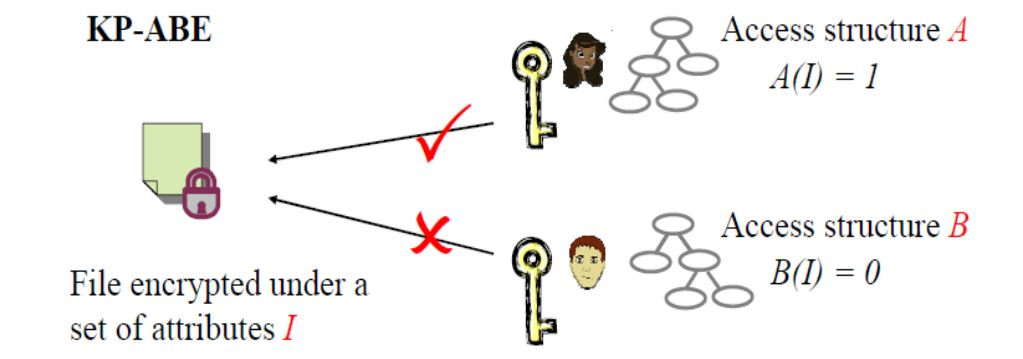
\includegraphics[width=\textwidth,height=7cm,keepaspectratio=true]{figures/KP-ABE.JPG}
    \caption{
        Key-Policy Attribute based Encryption visual representation from \cite{ka}
    }
	\end{figure}
  \end{center}

  \item \textit{Cipher-Policy Attribute based Encryption} is a policy that appeared after the classical KP-ABE but it is simpler and more natural than the previous construction that is more suited for complex access structures. This policy takes in the \textit{encryption} phase a access structure and the resource that needs to be encrypted (notice that the KP-ABE takes as input the attributes) and the security parameters given by the \textit{setup} phase. Then, in the \textit{key generation}/\textit{decryption} phases, the user takes his attributes and uses them with the access structure of the resource in order to gain access: if his attributes and the resource structure match, he can generate the decryption key and thus he gains access to that resource, otherwise the access is denied (he cannot generate the decryption key - see \textit{Figure 2}).

  \begin{center}
  	\begin{figure}[htpb]
    \centering
    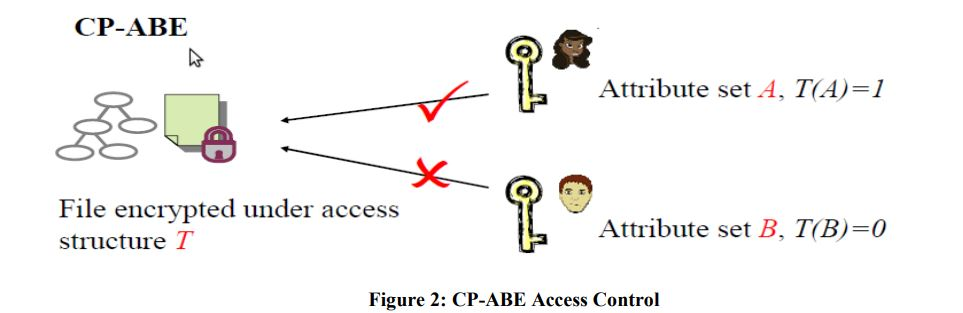
\includegraphics[width=\textwidth,height=7cm,keepaspectratio=true]{figures/CP-ABE.JPG}
    \caption{
        Cipher-Policy Attribute based Encryption visual representation from \cite{ka}
    }
	\end{figure}
  \end{center}
\end{itemize}

\subsection{Bilinear maps}

Let $G_1$ and $G_2$ two multiplicative cyclic groups of prime order $p$ and a function $e : G_1 \times G_1 \leftarrow G_2$. The function $e$ is called bilinear map if:

$$e(x^a, y^b) = e(x, y)^{ab}, \forall x, y \in G_1 \textrm{ and } a, b \in \mathbb{Z}_p \textrm{ and,}$$

$$e(g, g) \textrm{ is a generator of } G_2, \forall g \textrm{ generator of } G_1$$

The \textbf{jPBC} library provides costruction of bilinear maps from eliptic curves by specifing the type of curve that you intend to use. It has support for different types of curves like $A$ curves($y^2 = x^3 + x$), curves based on \textit{Diophantine} equation, etc.. The class that represents a bilinear map is called \textit{Pairing} in \textbf{jPBC} and you can instatiate this class using the following (example for $A$ type curve):

\begin{lstlisting}
PairingFactory.getPairing(new TypeACurveGenerator(rBits, qBits)
			  .generate())
\end{lstlisting} 

where the rBits and qBits are the curve parameters. For other curves the parameters may be different, but the idea is that you can use the \textit{PairingFactory} class to generate the desired bilinear map. You can also specify in a file other types of bilinear maps derived from the \textbf{PBC} library and currently there are not known any compatibility issues.

To apply a bilinear map to some given elements of $G_1$, $element_1, element_2$ you can achive that by using the following code:

\begin{lstlisting}
Element result = pairing.pairing(element1, element2);
\end{lstlisting} 

Some other useful operations might be:

\begin{lstlisting}
// get the Z_r field object
Field zr = pairing.getZr();

// get G_1 field object
Field g1 = pairing.getG1();

// new random element from Z_r
Element e1 = zr.newRandomElement();

// new identity element of Z_r
Element e2 = zr.newOneElement();

// new zero element of Z_r
Element e3 = zr.newZeroElement();

// addition, multiplication, pow
e1.add(e2);
e1.mul(e2);
e1.powZn(e2);
\end{lstlisting} 

\subsection{Decisional Bilinear Diffie-Hellman assumption}

Let $G_2$ be a bilinear group of order $p$ and $g$ a generator of this group. The \textit{Decisional Bilinear Diffie-Hellman assumption}(DBDH assumption) states that given $g^a, g^b, g^c, g^z$ where $a, b, c, z \in \mathbb{Z}_p$ randomly chosen and $g$ is the generator of group $G_1$, you can't distinguish from $e(g, g)^{abc}$ and $e(g, g)^z$ using a \textit{probabilistic polynomial-time} algorithm for the elements of $G_2$.

We'll use the \textit{DBDH assumption} for the security proof our extension.

\subsection{Boolean circuits}

A \textbf{boolean circuit} is a mathematical model that represents tree (binary in its classic form) where the leaf nodes are considered input values (\textit{boolean values} - \textit{true} or \textit{false}), the internal nodes represent boolean functions like \textit{OR, AND, NOT}. To evaluate this tree, one has to give the values to the input nodes and then traverse bottom-up the tree and for each node, look at its children values, apply the function defined for that node and update the circuit with its result. 

In this paper we'll focus on \textit{monotone boolean circuits} that means that thea are not allowed \textit{NOT} gates, but that does not consitute a loss of generality (see \cite{gghsw}). Also, the gates used in this paper have the following restricion: all the input gates have exactly one output wire (fan-out one), this is not a limitation because as proposed in \cite{fltccd} there can be used the \textit{Fan-Out gates} to achive a fan-outs greater than one for any gate (inclsively input gates). The FO-gates are a special type of gates with exactly one input and can have any number of outputs (any fan-out number) and what are these gates doing is that propagates the input values to the output values.

\subsubsection{Threshold gates}

The \textit{Threshold gates} come as an extension of the usual \textit{boolean circuits} gates $OR$ and $AND$ gates. A $(k, N)$ threshold gate represent a logical gate that have as input N values and in order to be evaluated as $true$ it has to have at least $k$ values from the input evaluated as $true$, otherwise the result of this gate is evaluated as $false$. For example, a $OR$ gate can be viewed as a $(1, 2)$ gate and a $AND$ gate can be viewed as a $(2, 2)$ gate.

\subsubsection{Example}

For the \textit{boolean circuit} in \textit{Figure 3} if the input of the gates is $[false, false, true, true]$, then result of the circuit will be $true$ because the gate $6^{th}$\textit{ gate(AND)} gate will be evaluated as $true$ and then the $8^{th}$\textit{ gate (OR)} gate will also be $true$.

If the input is $[true, false, false, true]$ the result of the circuit will be $false$ because the  $5^{th}$\textit{ gate (OR)} is evaluated as $false$, the $6^{th}$\textit{ gate (AND)} is evaluated with $false$, the $7^{th}$\textit{ gate (AND)} is evaluated as $false$ and as result the $8^{th}$\textit{ gate (OR)} will be evaluated with $false$.

\begin{center}
	\begin{figure}[htpb]
\centering
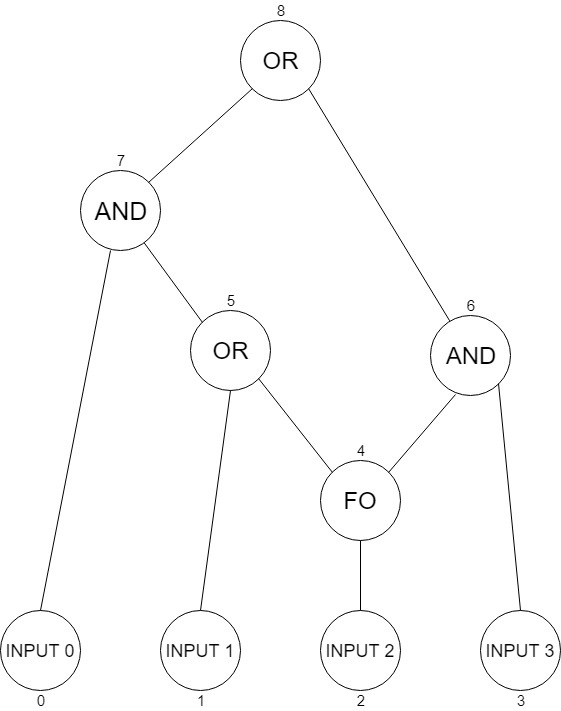
\includegraphics[width=\textwidth,height=8cm,keepaspectratio=true]{figures/boolean-circuit-fltccd.jpg}
\caption{
    Boolean circuit exmple that was also proposed in \cite{fltccd}
}
\end{figure}
\end{center}

The code that generates the boolean circuit above where $n$ is the number of inputs and $q$ is the number of internal gates:

\begin{lstlisting}
// regular gates
circuit = new DefaultCircuit(n, q, 3, new DefaultGate[]{
        new DefaultGate(INPUT, 0, 1),
        new DefaultGate(INPUT, 1, 1),
        new DefaultGate(INPUT, 2, 1),
        new DefaultGate(INPUT, 3, 1),

        new DefaultGate(FO, 4, 2, new int[]{2}),
        new DefaultGate(OR, 5, 3, new int[]{1, 4}),
        new DefaultGate(AND, 6, 3, new int[]{3, 4}),
        new DefaultGate(AND, 7, 4, new int[]{0, 5}),
        new DefaultGate(OR, 8, 3, new int[]{6, 7})
});

// threshold gates
circuit = new DefaultCircuit(n, q, 3, new DefaultGate[]{
        new DefaultGate(INPUT, 0, 1),
        new DefaultGate(INPUT, 1, 1),
        new DefaultGate(INPUT, 2, 1),
        new DefaultGate(INPUT, 3, 1),

        new DefaultGate(FO, 4, 2, new int[]{2}),
        new DefaultGate(KN, 5, 3, new int[]{1, 4}, 1),
        new DefaultGate(KN, 6, 3, new int[]{3, 4}, 2),
        new DefaultGate(KN, 7, 4, new int[]{0, 5}, 2),
        new DefaultGate(KN, 8, 3, new int[]{6, 7}, 1)
});
\end{lstlisting} 

\subsection{The Backtracking Attack}



\subsection{Adi Shamir's secret sharing algorithm}

The Shamir's secret sharing procedure was proposed first on \cite{shamir}(1979) and is strongly related to the \textit{threshold gates} described above. This schema proposes a way of sharing a secret $S$ using $S_1, S_2, ..., S_n$ pieces of $S$ and sharing them with $n$ entities and allow the secret $S$ to be reconstructed \textit{if and only if} at least $k, k \le n$ entities know their $S_{i_1}, S_{i_2}, ..., S_{i_k}$ pieces of the $S$ secret. 

\subsubsection{Algorithm}

Let $S$ be a number representing secret that has to be shared, $k$ be the number of entities required for the secret reconstruction and $N$ the total number of entities. To divide $S$ into $N$ pieces $S_1, S_2, ..., S_N$ the algorithm picks a random polynomial $p(x) = a_0 + a_1 * x + ... + a_{k - 1} * x^{k - 1}$ of $k - 1$ degree where $a_0$ represents $S$ (notice that $a_1, ..., a_{k - 1}$ must be random generated numbers) and then assign to each $S_i = p(i), \forall i = {1, 2, ... n}$.

In order to reconstruct the secret $S$ one has to know at least $k$ values of this polynomial and apply a interpolation algorithm in order to discover the $p(0)$ value and thus the $S$ value. The correctness comes from the sharing phase where for any $k$ values in a \textit{Euclidian space} there exists a unique polynomial of degree $k - 1$ that is discovered using the interpolation algorithm.

\subsubsection{Lagrange polynomial}

The \textbf{Lagrange polynomial} is used in \textit{computer science} and \textit{numerical analysis} as a interpolation technique that aproximates the lowest degree polynomial that satisfies the constraint that all the given points for interpolation are exactly matched by the output of this polynomial.

\textbf{Algorithm:} given a set of entries $(x_1, y_1), (x_2, y_2), ..., (x_n, y_n) \in \mathbb{R}^2$ the value of the Lagrange polynomial of degree $n$ in $x$ is given by the formula:

$$L^n(x) = \sum_{i = 0}^n(y_i\prod_{j \neq i, j = 0}^n \frac{x - x_j}{x_i - x_j})$$

This method can be used with the $S_{i_1}, S_{i_2}, ..., S_{i_k}$ from the Shamir secret sharing algorithm in order to compute the value $p(0)$ of the random generated polynomial and thus achieving the secret $S$.

\section{Extension for the KP-ABE schema based on bilinear maps using boolean circuits with threshold gates}

\subsection{Proposed schema}

\subsubsection{Description}
\subsubsection{Correctness}
\subsubsection{Complexity}

\subsection{Security proof}

\subsection{Applications}

\subsection{Implementation}

\section{Conclusions}

\pagebreak

\blankpage

\begin{thebibliography}{9}

\bibitem{fltccd} 
Ferucio Laurențiu Țiplea, Constantin Cătălin Drăgan, 
\textit{Key-policy Attribute-based Encryption for Boolean Circuits from Bilinear Maps}, 2014.

\bibitem{gghsw} 
Sanjam Garg, Craig Gentry, Shai Halevi, Amit Sahai, Brent Waters 
\textit{Attribute-Based Encryption for Circuits from Multilinear Maps}, 2013
 
\bibitem{gpsw} 
Vipul Goyal, Omkant Pandey, Amit Sahai, Brent Waters 
\textit{Attribute-Based Encryption for Fine-Grained Access Control of Encrypted Data}, 2006

\bibitem{ggh}
Sanjam Garg, Craig Gentry, Shai Halevi
\textit{Candidate Multilinear Maps from Ideal Lattices}, 2012

\bibitem{msz}
Eric Miles, Amit Sahai, Mark Zhandry
\textit{Annihilation Attacks for Multilinear Maps:Cryptanalysis of Indistinguishability Obfuscation over GGH13}, 2016

\bibitem{shamir}
Adi Shamir
\textit{How to Share a Secret}, 1979

\bibitem{blakley}
G. R. Blakley
\textit{Safeguarding cryptographic keys}, 1899

\bibitem{brickell}
E. F. Brickell
\textit{Some ideal secret sharing schemes. Journal of Combinatorial Mathematics and Combinatorial Computing}, 1989

\bibitem{isn}
M. Ito, A. Saito, and T. Nishizeki
\textit{Secret Sharing Scheme Realizing General Access Structure}, 1987

\bibitem{jpbc}
Angelo {De Caro} and Vincenzo Iovino
\textit{jPBC: Java pairing based cryptography Library}, 2011

\bibitem{pbc}
Ben Lynn
\textit{Pairing based cryptography library}

\bibitem{gmp}
\href{https://gmplib.org/\#WHAT}{https://gmplib.org/\#WHAT}
\textit{The GNU Multiple Precision Arithmetic Library}

\bibitem{bc}
\href{https://www.bouncycastle.org/about.html}{https://www.bouncycastle.org/about.html}
\textit{The Legion of the Bouncy Castle}

\bibitem{gghvv}
Craig Gentry, Sergey Gorbunov, Shai Halevi, Vinod Vaikuntanathan, Dhinakaran Vinayagamurthy
\textit{How to Compress (Reusable) Garbled Circuits}, 2013

\bibitem{shamirid}
Adi Shamir
\textit{Identity-Based Cryptosystems and Signature Schemes}, 1984 

\bibitem{sok}
Sakai R., Ohgishi K., Kasahara M.
\textit{Cryptosystems based on pairings}, 2000 

\bibitem{bf}
Dan Boneh, Matt Franklin
\textit{Identity-based encryption from the Weil pairing}, 2001

\bibitem{ka}
Parmar Vipul Kumar J, RajaniKanth Aluvalu
\textit{Key Policy Attribute Based Encryption (KP-ABE): A Review}, 2015

\bibitem{idwiki}
\href{https://en.wikipedia.org/wiki/ID-based_encryption}{https://en.wikipedia.org/wiki/ID-based\_encryption}

\bibitem{abecryptostack}
\href{https://crypto.stackexchange.com/questions/17893/what-is-attribute-based-encryption?utm_medium=organic&utm_source=google_rich_qa&utm_campaign=google_rich_qa}{https://crypto.stackexchange.com/questions/17893/}

\bibitem{abewiki}
\href{https://en.wikipedia.org/wiki/Attribute-based_encryption}{https://en.wikipedia.org/wiki/Attribute-based\_encryption}

\bibitem{bilinearmapwiki}
\href{https://en.wikipedia.org/wiki/Bilinear_map}{https://en.wikipedia.org/wiki/Bilinear\_map}

\bibitem{dbdhwiki}
\href{https://en.wikipedia.org/wiki/Decisional_Diffie\%E2\%80\%93Hellman_assumption}{https://en.wikipedia.org/wiki/Decisional\_Diffie\%E2\%80\%93Hellman\_assumption}

\bibitem{booleancircuitwiki}
\href{https://en.wikipedia.org/wiki/Boolean_circuit}{https://en.wikipedia.org/wiki/Boolean\_circuit}

\bibitem{shamirwiki}
\href{https://en.wikipedia.org/wiki/Shamir\%27s_Secret_Sharing}{https://en.wikipedia.org/wiki/Shamir\%27s\_Secret\_Sharing}

\bibitem{lagrangewiki}
\href{https://en.wikipedia.org/wiki/Lagrange_polynomial}{https://en.wikipedia.org/wiki/Lagrange\_polynomial}

\end{thebibliography}

\vspace{\baselineskip}

\end{document}